% !TeX root = ../main.tex

\chapter{文獻探討}

為了建構一套兼具低成本與高效能的多功能樂高螢光倒立式顯微鏡，本研究廣泛參考了光學工程、機電整合、電腦視覺與運算成像等多個領域的先驅研究與基礎理論。本章針對開源硬體顯微鏡的發展現況、自動對焦技術的演進、影像感測器的底層物理機制，以及運算成像與傅立葉疊層的數學基礎進行深度的探討。

\section{開源硬體顯微鏡的發展與機構分析}

隨著自造者運動（Maker Movement）的興起，學術界開始致力於打破高階儀器的壟斷，推動「硬體民主化（Hardware Democratization）」。在開源顯微鏡領域，有幾個極具代表性的專案，它們各自提出了不同的機械與光學解決方案。

\subsection{OpenFlexure Microscope 與撓性機構的力學原理}

由英國巴斯大學（University of Bath） Richard Bowman 團隊開發的 OpenFlexure Microscope \citep{collins2020robotic} 是目前開源硬體領域最具代表性的 3D 列印顯微鏡，如圖 \ref{fig:openflexure} 所示。其核心技術創新在於採用了「單體式 3D 列印撓性機構（Monolithic 3D-printed flexure-based mechanism）」。該機構利用塑膠材料的彈性特性，透過四連桿平行撓性結構的微小變形來驅動載台。根據文獻報告，該系統配合標準 M3 螺栓與小型減速步進馬達，能達成 Z 軸高達 50 nm、X-Y 軸達 70 nm 的精密步進位移，展現出足以應對高倍率顯微觀測的定位能力。

\begin{figure}[H]
    \centering
    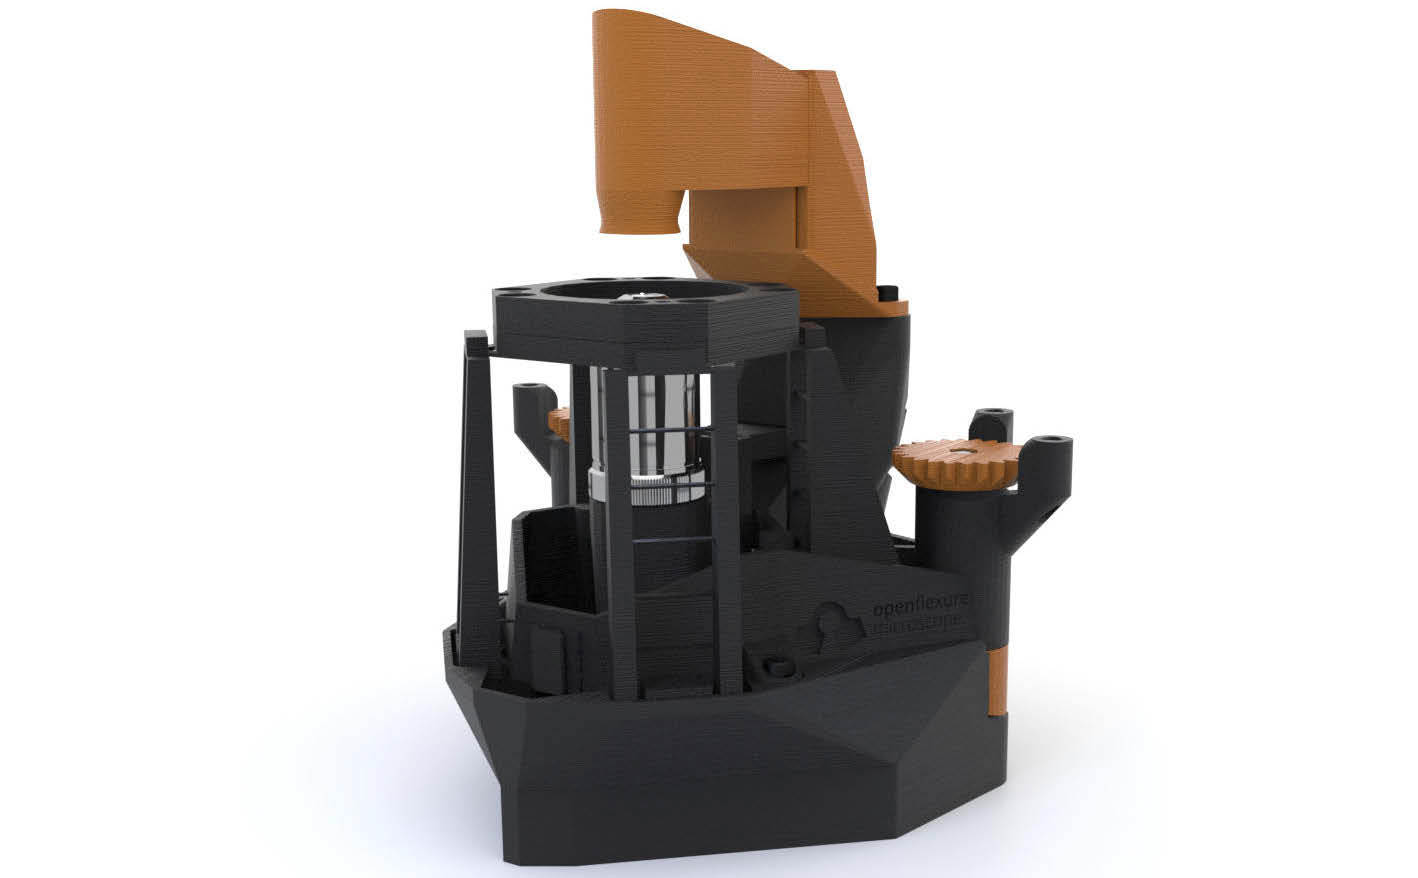
\includegraphics[width=0.8\textwidth]{figures/fig2_6_openflexure.png}
    \caption{OpenFlexure Microscope 之機身架構圖，展示了其一體成型的 3D 列印機構設計（圖片來源：\citep{collins2020robotic}）。}
    \label{fig:openflexure}
\end{figure}

這種撓性機構的設計初衷，是為了從根本上消除傳統機械結構中的背隙（Backlash）與靜摩擦力（Stiction）問題。在傳統的金屬加工載台中，物體移動依賴滑軌與齒輪間的相對運動，不可避免地會產生機械空隙與「粘滑效應（Stick-slip）」。OpenFlexure 則透過 3D 列印將整個位移機構整合為連續的固體物理連接，在特定的力學節點處縮減壁厚以形成撓性鉸鏈（如圖 \ref{fig:flexure_issue} 所示）。由於不存在任何分離的滑動面，該機構能達成絕對零背隙的平滑運動，這對於自動化對焦與高精度掃描至關重要。

\begin{figure}[H]
    \centering
    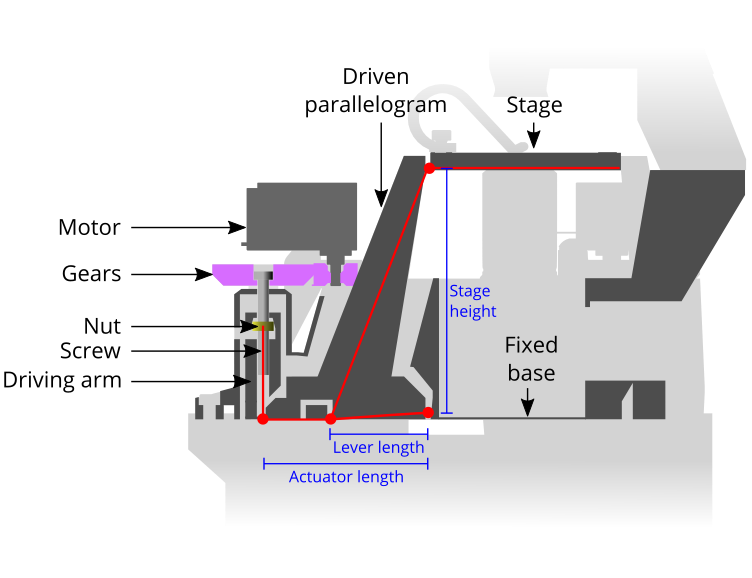
\includegraphics[width=0.8\textwidth]{figures/fig2_7_flexure_issue.png}
    \caption{撓性機構（Flexure Mechanism）之微米級位移原理與材料受力點分析圖。}
    \label{fig:flexure_issue}
\end{figure}

然而，撓性機構也面臨顯著的物理限制。首先，位移行程受限於材料的彈性變形區間，OpenFlexure 的典型行程僅約為 12 $\times$ 12 $\times$ 4 mm，較傳統機械載台小得多，限制了大面積樣本的掃描能力。其次，根據胡克定律（Hooke's Law），若位移量過大導致材料應力超過降服強度，將產生不可逆的塑性形變。此外，全塑膠結構的機械剛性較低，容易受到環境振動影響，且在長時間負載下會產生應力潛變（Creep），導致光軸漂移。正是基於對上述穩定性與行程限制的考量，本研究決定選擇揚棄撓性機構，改採具備更高剛性的自動化位移平台架構。

\newpage
\subsection{Incubot 系統分析}
\textbf{Incubot} \citep{merces2021incubot} 是一款改裝自消費級 3D 印表機機架的小型顯微鏡，其特色在於機身極簡且低成本。然而，該系統在功能上有顯著侷限：它僅針對明視野（Bright-field）成像設計，並不具備螢光觀測能力。在光路建構上，其光源採用矽膠（Silicone）進行簡易固定，這種非剛性的固定方式在培養箱的高溫潮濕環境下，極易因材料軟化或應力變化導致照明光軸偏移，難以維持長期的光路準直性，如圖 \ref{fig:incubot} 所示。

\begin{figure}[H]
    \centering
    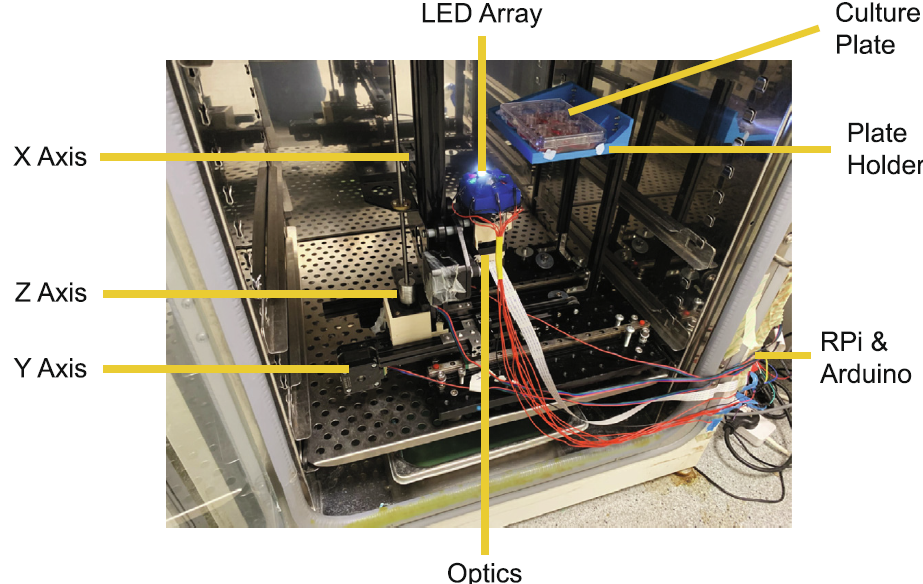
\includegraphics[width=0.8\textwidth]{figures/fig2_8_incubot.png}
    \caption{Incubot 系統架構圖，展示了其基於 3D 印表機框架的簡易設計（圖片來源：\citep{merces2021incubot}）。}
    \label{fig:incubot}
\end{figure}

\newpage
\subsection{UC2 模組化系統}
\textbf{UC2 (Use-Case-box)} \citep{diederich2020versatile} 則是另一款極具啟發性的設計。UC2 採用了「方塊積木」的概念，將雷射、透鏡、相機等光學元件分別裝入標準尺寸的 3D 列印方塊中。研究人員可以像拼圖一樣將這些方塊組合在帶有磁鐵的底板上。雖然 UC2 提供了高度的擴充性，但其磁吸底板的定位精度與整體結構剛性，在面對需要頻繁移動載台的自動化掃描時，仍顯得力不從心，如圖 \ref{fig:uc2} 所示。

\begin{figure}[H]
    \centering
    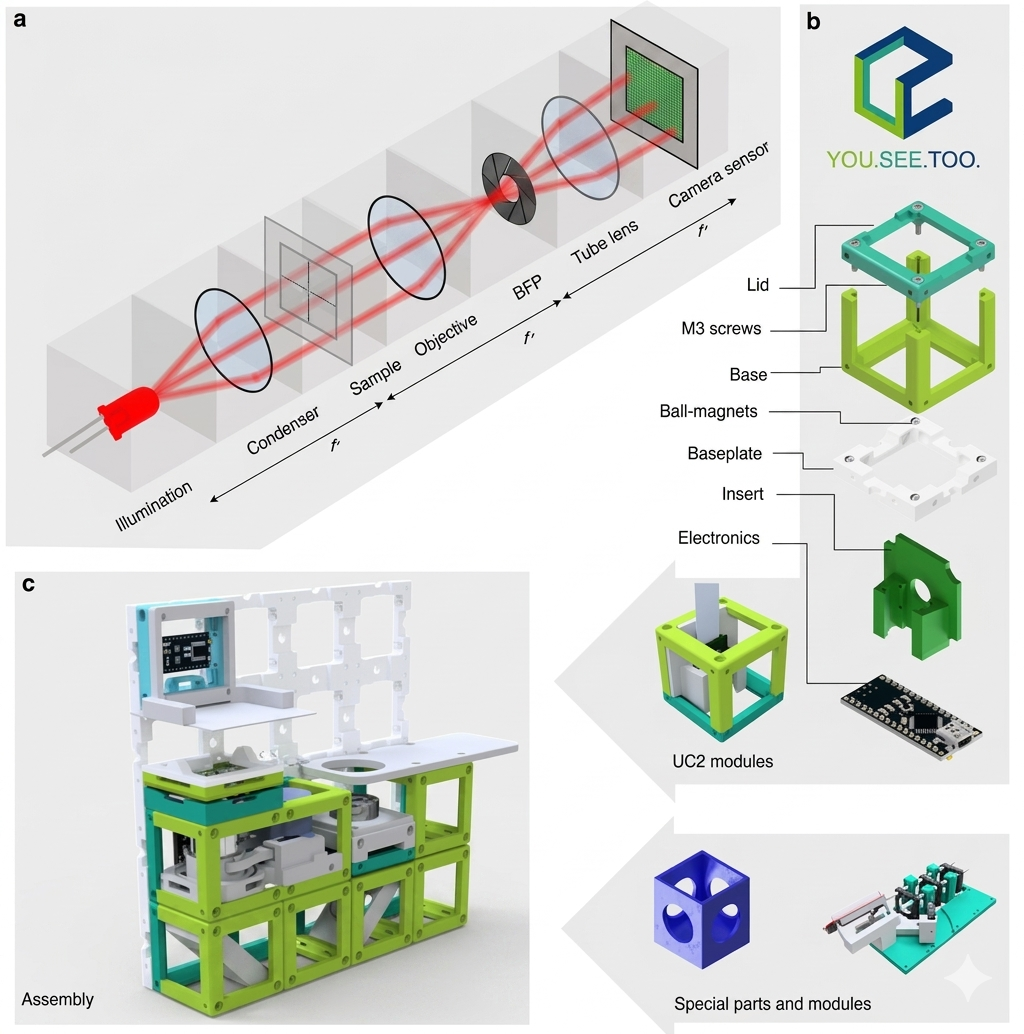
\includegraphics[width=0.8\textwidth]{figures/fig2_9_uc2.png}
    \caption{UC2 模組化系統，展示了其磁吸式方塊光學元件設計（圖片來源：\citep{diederich2020versatile}）。}
    \label{fig:uc2}
\end{figure}

\newpage
\subsection{IBM Lego Microscope：工業級積木的精密應用}
由 IBM 蘇黎世研究實驗室研究員 Yuksel Temiz 所開發的樂高顯微鏡 \citep{temiz2020lego}，是開源硬體領域中將「消費級積木」推向「實驗室等級儀器」的標竿案例。該專案的核心理念是利用樂高科技系列（Lego Technic）積木極高的工業製造精度誤差小於 $10 \mu m$ \citep{temiz2020lego}，建構出一套具備高剛性且可重複配置的顯微鏡架構。

在硬體架構上，該系統採用正立式（Upright）光路配置，整合了 Raspberry Pi 作為影像處理核心，並透過 Arduino 控制多個步進馬達，達成自動化的樣本移動與對焦控制。值得注意的是，該系統主要針對明視野成像與微流道實驗設計，並不具備螢光觀測功能。Temiz 的研究證明，透過合理的幾何桁架設計，樂高積木足以支撐標準的高倍率顯微物鏡，並在微流道（Microfluidics）實驗中精準捕捉液滴運動（如圖 \ref{fig:ibm_microscope} 所示）。相較於 3D 列印機構可能存在的層間誤差與材料老化變形，樂高積木的射出成型穩定性提供了一種更為強健、且易於在全球範圍內複製的精密機械解決方案，這也為本研究選擇樂高作為核心架構提供了重要的理論支持。

\begin{figure}[H]
    \centering
    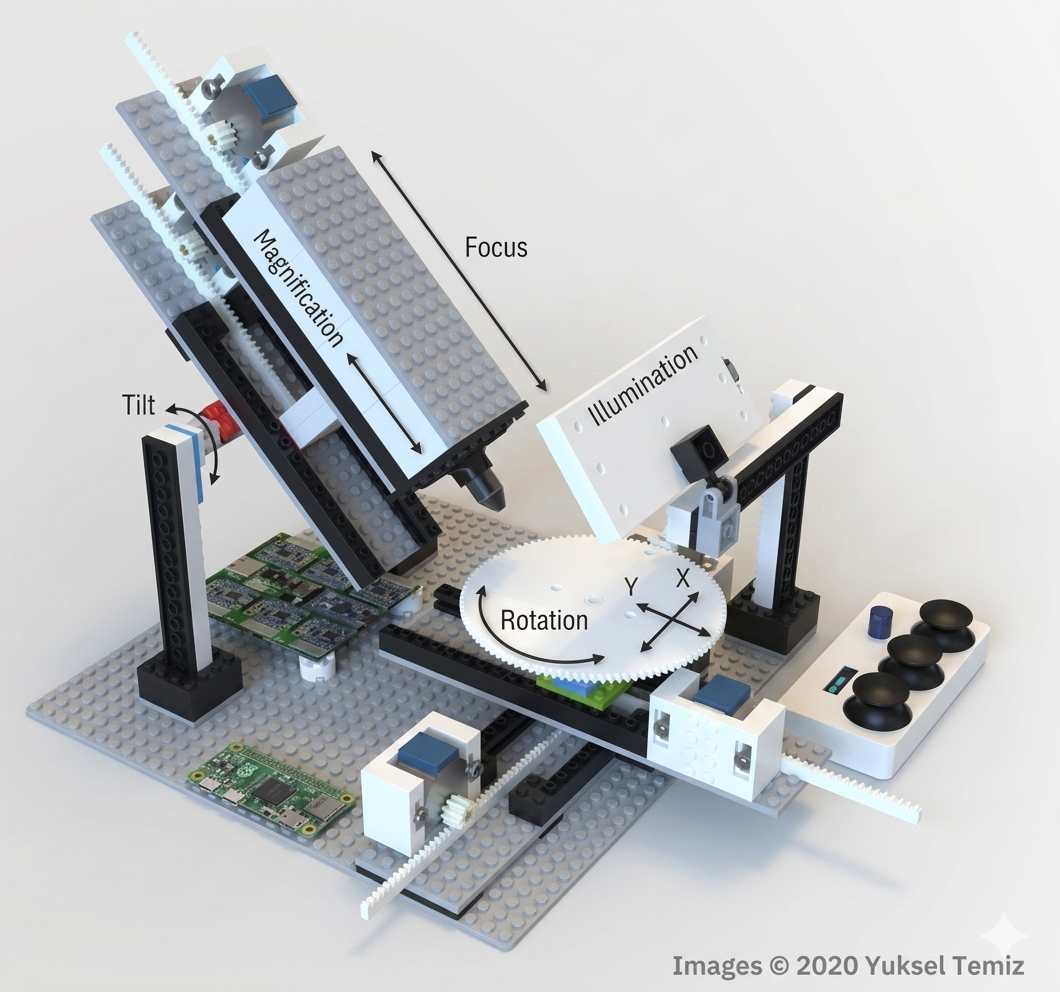
\includegraphics[width=0.8\textwidth]{figures/fig2_10_ibm_microscope.png}
    \caption{IBM Lego Microscope 系統架構圖，展示了利用樂高科技系列積木構建的高精度顯微機身（圖片來源：\cite{temiz2020lego}）。}
    \label{fig:ibm_microscope}
\end{figure}

綜合上述文獻，我們可以發現：現有的開源設計在「低成本」、「高精度」、「大行程」與「高剛性」這四個維度上始終無法兼顧。本研究正是試圖透過樂高積木的工業級精度與龍門機電架構，找到這四者的最佳平衡點。

\newpage
\section{自動對焦搜索演算法之演進}

在自動化顯微掃描過程中，焦平面會隨樣本不平整或機構運動而產生微米級的偏移，因此一套兼顧效率與精度的自動對焦（Autofocus, AF）演算法至關重要。傳統的對焦搜索多採用單純的登山演算法（Hill-climbing algorithm），但在複雜樣本下容易陷入局部極大值（Local Maximum），且固定步長的設計往往無法在搜索速度與精度之間取得平衡。

Fu 等人 \cite{fu2015fast} 針對此問題提出了一種基於改進型登山搜索（Improved Mountain-climb Searching, MCS）的快速自動對焦方法。該研究的核心改進邏輯可總結為以下三個維度。首先是引入「自適應步長」以跳過雜訊干擾區。傳統爬山演算法若使用固定小步長，極易被影像雜訊產生的微小峰值誤導。該研究設計的第一步步長 $step_1$ 與起始位置的圖像評價函數值成反比，其公式原理為 $step_1 = \text{round}(k / F_{var}(I_0))$。當系統處於嚴重離焦時，方差評價函數 $F_{var}$ 值很小，計算出的 $step_1$ 就會非常大。這個較大的初次步長能讓鏡頭直接「跳過」山腳下由雜訊引起的局部小峰值，快速抵達接近山腰的主峰斜率區。

\begin{figure}[H]
    \centering
    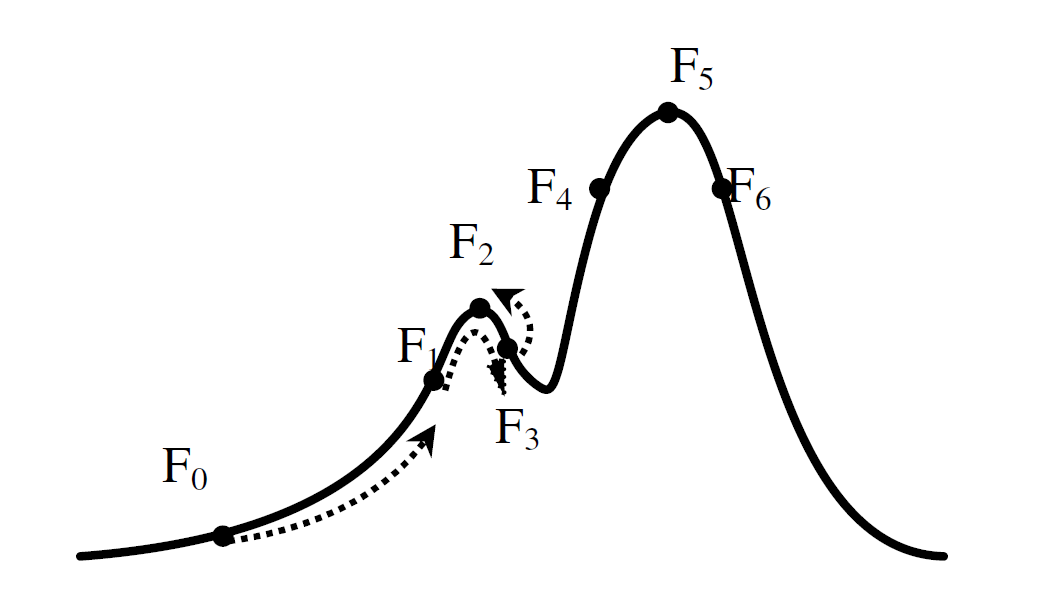
\includegraphics[width=0.75\textwidth]{figures/MCS algorithm.png}
    \caption{改進型登山搜索之焦平面搜索邏輯示意圖（參考自 \cite{fu2015fast}）。}
    \label{fig:mcs_algorithm}
\end{figure}

其次是雙評價函數的「粗精結合」策略。研究分析發現不同的評價函數具備不同的曲線特性，為了應對局部極大值，系統將兩種函數結合使用：在粗對焦階段採用「方差函數（Variance）」，因其曲線峰值範圍較寬且在遠離焦點處較為平滑，有利於在大範圍內尋找主峰方向；在精對焦階段則切換至「Brenner 梯度函數」，其曲線極其陡峭且靈敏度高，能精確鎖定真正的全域最大值。如圖 \ref{fig:mcs_metrics_10x} 所示，這套邏輯確保了系統能在不同焦距範圍下切換最適用的評價指標。

\begin{figure}[H]
    \centering
    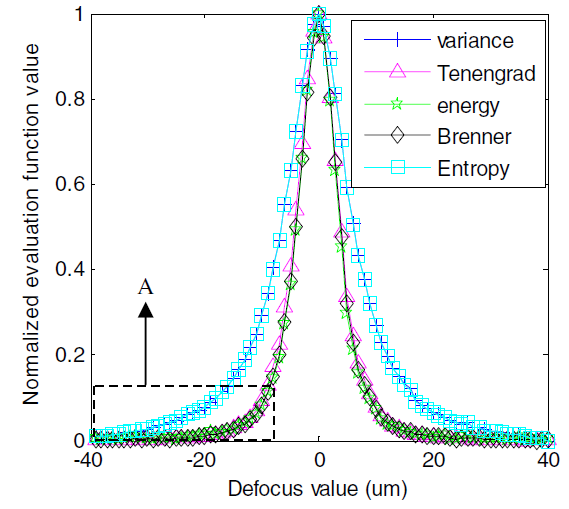
\includegraphics[width=0.75\textwidth]{figures/MCS focus metrics 10x.png}
    \caption{在 10 倍物鏡下不同對焦評價函數之效能比較圖（MCS Metrics Comparison）。}
    \label{fig:mcs_metrics_10x}
\end{figure}

最後，在搜索流程中引入了判定門檻值 $\Delta F_0$。如圖 \ref{fig:mcs_flowchart} 的演算法流程圖所示，當第一步 $step_1$ 走完後，若評價函數值的變化量小於 $\Delta F_0$，系統會判定目前可能落入了局部極大值的平緩區域。此時系統會強迫沿著爬坡方向再額外跨出一個「雙倍 $step_1$」的步長，以確保鏡頭能衝出雜訊干擾，進入真正的上升路徑。

\begin{figure}[H]
    \centering
    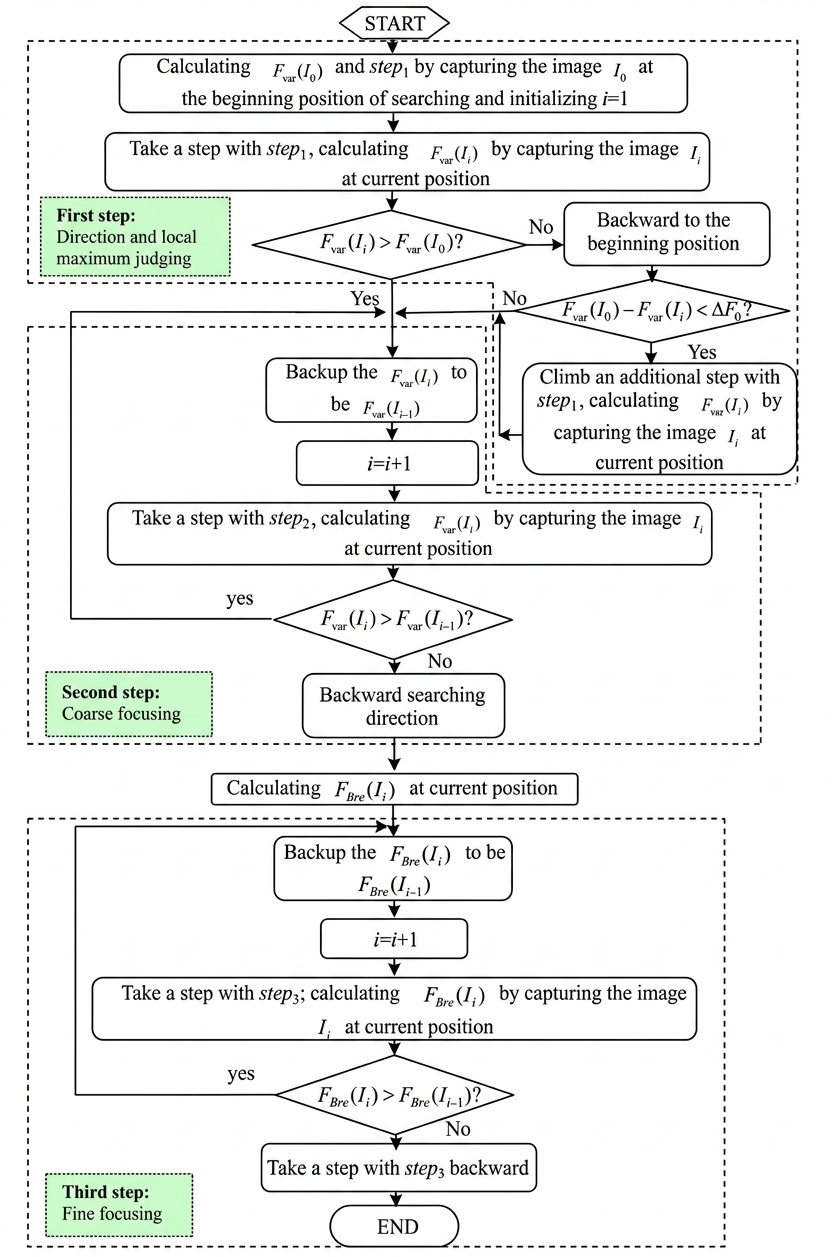
\includegraphics[width=0.75\textwidth]{figures/MCS flow chart.png}
    \caption{改進型登山搜索之演算法執行流程圖（參考自 \cite{fu2015fast}）。}
    \label{fig:mcs_flowchart}
\end{figure}


透過上述「大步跨越雜訊、小步鎖定精確峰值」的邏輯，該演算法在血塗片（Leukocyte）等背景複雜的樣本檢測中展現出較強的穩健性。然而，進一步分析該演算法可以發現，其效能高度依賴於對特定類型樣本與硬體環境的預先調優。具體而言，關鍵參數如自適應步長的比例係數 $k$ 與判定門檻值 $\Delta F_0$ 通常是基於特定樣本的「已知數字變化」而設定的。這種設計導致了泛用性的缺失：一旦樣本類型更換（例如從血塗片改為螢光細胞），原有的參數設定將不再適用，可能導致自適應步長失效或誤判門檻，進而使演算法失去其預期的效率。正是基於對此局限性的考量，本研究在後續實作自動化系統時，將演算法進行優化，以符合不同樣本的適用性。

\newpage
\section{感測器物理學與色彩校正 (Color Correction) 理論}

將百元等級的 Raspberry Pi Camera 取代數十萬元科學級相機的代價，就是必須面對消費級感測器在光學設計上的嚴重妥協。現代 CMOS 感測器為了極致的微縮化，其每一個感光像素（Pixel）的面積極小。為了提高感光度，半導體工程師會在每一個像素上方製作一個微小凸透鏡，稱為**微透鏡陣列（Microlens Array）**。這些微透鏡負責將照射到像素邊緣的光線「匯聚」到像素中心的感光區。

然而，微透鏡的聚光角度是經過精心計算的，它必須與原廠搭配的鏡頭的主光線角度（CRA）完美匹配。通常，智慧型手機鏡頭邊緣射入感測器的光線會帶有一個傾斜角度。當我們將 Raspberry Pi Camera 的原廠小鏡頭拔除，換上顯微鏡的「有限共軛系統」時，顯微光路投射到感測器邊緣的光線通常是近乎垂直的（CRA 接近 0 度）。這就導致了災難性的後果：垂直入射的顯微光線，在經過感測器邊緣的傾斜微透鏡時，被錯誤地折射到了該像素的「感光區之外」，甚至是折射到了「隔壁的像素」裡，如圖 \ref{fig:cra_mismatch} 所示。

\begin{figure}[H]
    \centering
    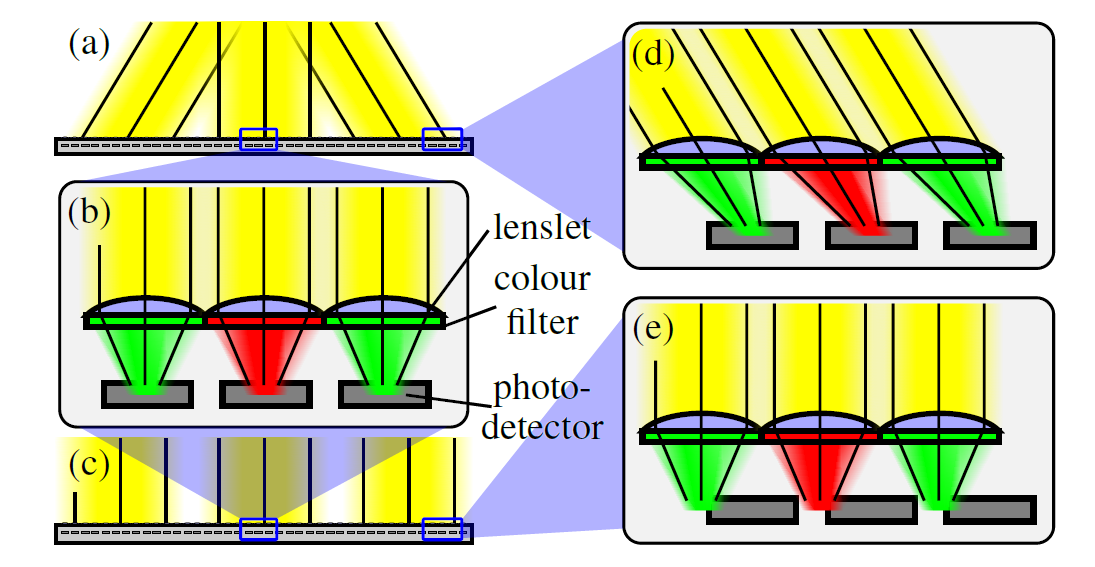
\includegraphics[width=0.8\textwidth]{figures/fig2_5_cra_mismatch.png}
    \caption{Raspberry Pi Camera 邊緣像素的主光線角度（CRA）錯位與色彩串擾示意圖（圖片來源：\cite{bowman2019flat}）。}
    \label{fig:cra_mismatch}
\end{figure}

上述的 CRA 不匹配直接導致了兩個致命的影像缺陷。首先是\textbf{嚴重暗角（Vignetting）}：畫面中心的光線垂直進入微透鏡，正確落在感光區，因此中心明亮；越靠近畫面邊緣，光線被錯誤折射流失得越多，導致影像邊緣變得極度暗沉。其次是\textbf{色彩串擾（Color Crosstalk）}：幾乎所有消費級彩色相機都覆蓋著拜爾濾波器（Bayer Filter Array, 依據 RGGB 排列），當綠色像素上的微透鏡將光線錯誤折射到隔壁的紅色或藍色像素時，感測器就會回報錯誤的顏色資訊。這使得原本應該是純綠色的螢光樣本，在影像周圍會因為光譜溢出而變成蒼白、甚至是紫紅色的錯誤色彩。

這些物理層面的缺陷無法透過改變顯微鏡的機械結構來修復。針對此一挑戰，Bowman 等人 \cite{bowman2019flat} 在其研究「Flat-field and colour correction for the Raspberry Pi camera module」中，提出了一套專為 Raspberry Pi Camera Module 設計的平場與色彩校正演算法。
唯一且最有效的方法，就是深入影像處理的底層，透過建立複雜的「空間變異增益矩陣（Spatially Varying Gain Maps）」與「解混張量（Unmixing Tensor）」，在每一個像素點上進行精準的反向數學補償。這正是本論文第三章「影像處理管線」將要詳細推導與實作的核心技術。

\newpage
\section{運算成像與圖案化照明傅立葉疊層 (piFP) 理論}

為了克服傳統顯微系統中的繞射極限限制，運算成像（Computational Imaging）技術提供了突破物理孔徑限制的新途徑。本節將概述傅立葉疊層成像（Fourier Ptychography, FP）的演進過程，及其如何從明視野成像擴展至螢光成像領域。

\subsection{傅立葉疊層成像 (Fourier Ptychography, FP) 的核心思想}
如果在明視野下高頻光線進不了物鏡，那我們能不能改變照明的角度？
FP 技術的核心思想最早由 Zheng 等人於 2013 年提出 \cite{zheng2013wide}：透過從不同角度（傾斜）照射樣本，強迫原本會發散到物鏡外的大角度高頻光線，被「推」進物鏡的接收錐角內。透過依次點亮 LED 陣列中不同位置的單元，我們可以拍攝一系列低解析度但包含不同頻譜資訊的影像。最後，利用疊代相位復原演算法（Iterative Phase Retrieval Algorithm），在電腦的頻域（Fourier Domain）空間中，將這些重疊的小區塊頻譜「縫合」成一個巨大無比的頻譜（系統架構如圖 \ref{fig:fp_setup} 所示），經由反傅立葉轉換後，即可獲得極高解析度的影像。

\begin{figure}[H]
    \centering
    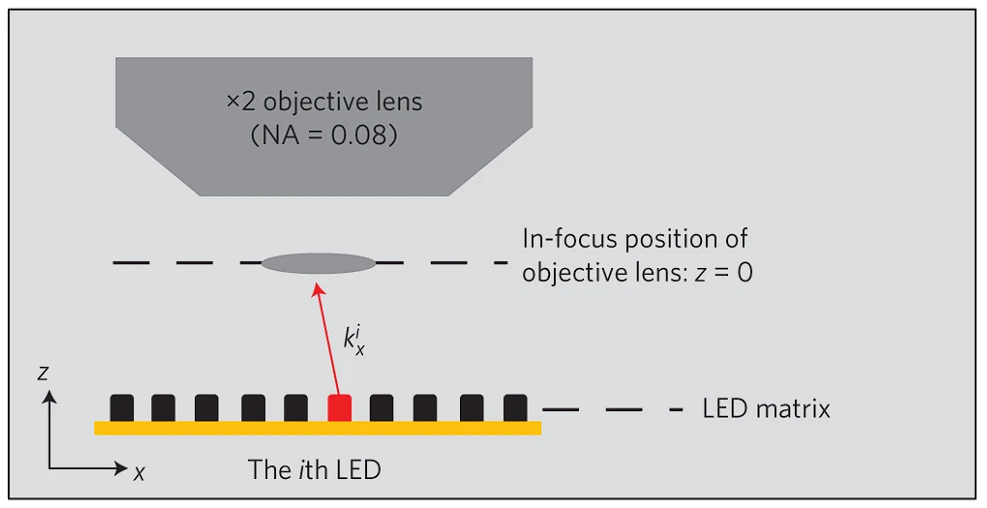
\includegraphics[width=0.8\textwidth]{figures/fig2_12_fp_setup.png}
    \caption{基於 LED 陣列之傅立葉疊層成像 (FP) 系統架構示意圖（圖片參考自 \cite{zheng2013wide}）。系統透過可程式化控制的 LED 陣列提供不同角度的照明，將樣本的高頻資訊偏移至物鏡可接收的孔徑內。}
    \label{fig:fp_setup}
\end{figure}

\subsection{基於擴散片波前調控之明視野 FP}
針對傳統 LED 陣列 FP 系統在硬體調校上的複雜性，He 等人 \citep{he2020fourier} 提出了一種僅需利用低成本擴散片（Diffuser）進行波前調控的改良方案（Fourier ptychography via wavefront modulation with a diffuser）。
該技術的核心在於：當照明光穿過擴散片後，會產生隨機的相位調控，強迫樣本的高頻資訊在通過物鏡前進行編碼。透過平移擴散片以產生一系列不同的隨機圖案影像，演算法便能從中還原出原本遺失的高頻細節，如圖 \ref{fig:pifp_setup_bf} 所示。

\begin{figure}[H]
    \centering
    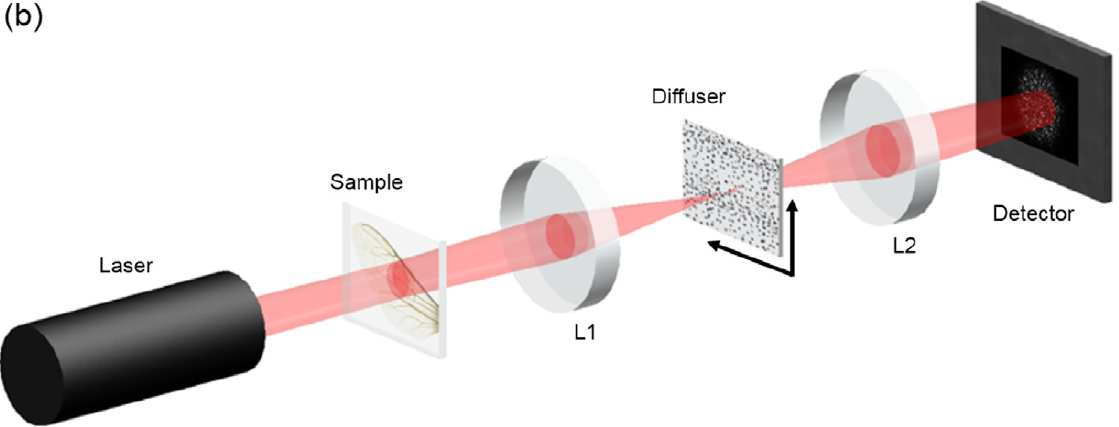
\includegraphics[width=0.8\textwidth]{figures/pifp_setup_bf.png}
    \caption{基於擴散片波前調控之明視野傅立葉疊層成像系統架構（圖片來源：\cite{he2020fourier}）。}
    \label{fig:pifp_setup_bf}
\end{figure}

\subsection{針對螢光系統的 piFP 與波前調控}
傳統的 FP 依賴 LED 陣列進行角度掃描，且必須建立在光線是「相干的（Coherent）」（如雷射或窄頻 LED）前提下。然而，螢光發光是一種「非相干（Incoherent）」且自發各向同性的過程，傳統的 FP 無法直接應用於螢光成像。
為此，Dong 等人提出了 \textbf{圖案化照明傅立葉疊層 (piFP)} \citep{dong2014high}。piFP 放棄了角度掃描，改為在樣本前方放置一個能夠產生空間高頻圖案（例如散斑 Speckle）的元件。
根據頻率混疊（Aliasing）原理，當我們將高頻的照明圖案疊加在樣本上時，照明圖案的空間頻率會與樣本的空間頻率發生相加或相減的「差頻效應」。這會將樣本極高頻的細節，硬生生地「搬移（Shift）」到低頻區域，使其能夠順利穿過低 NA 的物鏡被相機捕捉。
He 等人 \citep{he2020fourier} 進一步證實了使用低成本擴散片（Diffuser）進行波前調控的優越性。在我們的系統中，我們即是透過移動擴散片來產生不同的隨機圖案照明，藉由記錄多張帶有不同圖案混疊的螢光影像，最終在演算法中解譯出被隱藏的高解析度螢光結構。

\begin{figure}[H]
    \centering
    \begin{minipage}{0.48\textwidth}
        \centering
        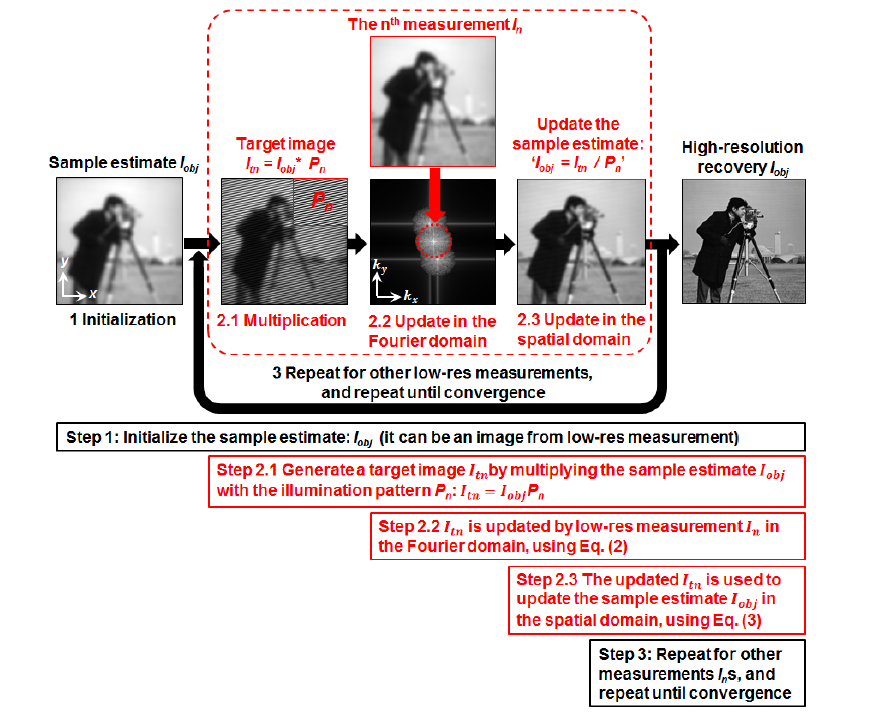
\includegraphics[width=\textwidth]{figures/fig2_13_pifp_concept.png}
        \caption{piFP 突破繞射極限之原理示意圖（圖片來源：\cite{dong2014high}）。}
        \label{fig:pifp_concept}
    \end{minipage}
    \hfill
    \begin{minipage}{0.48\textwidth}
        \centering
        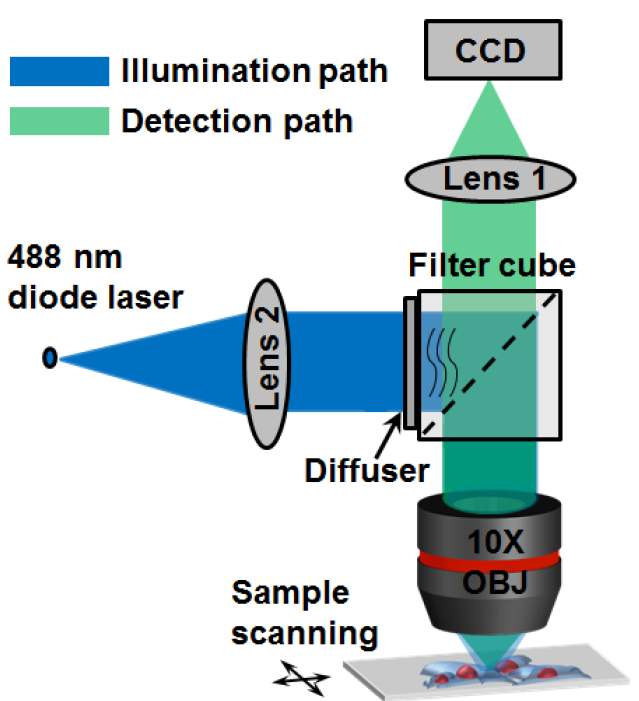
\includegraphics[width=\textwidth]{figures/pifp_setup_fluo.png}
        \caption{針對螢光系統的 piFP 實作架構示意圖。}
        \label{fig:pifp_setup_fluo}
    \end{minipage}
\end{figure}